\section{Protokoll för kommunikation}

\begin{figure}[H]
\center
\scalebox{0.6}{% Graphic for TeX using PGF
% Title: /home/hannes/GitHub/TSEA29/dokumentation/designspecifikation/FLOW1.dia
% Creator: Dia v0.97.2
% CreationDate: Thu Oct  9 16:44:50 2014
% For: hannes
% \usepackage{tikz}
% The following commands are not supported in PSTricks at present
% We define them conditionally, so when they are implemented,
% this pgf file will use them.
\ifx\du\undefined
  \newlength{\du}
\fi
\setlength{\du}{15\unitlength}
\begin{tikzpicture}
\pgftransformxscale{1.000000}
\pgftransformyscale{-1.000000}
\definecolor{dialinecolor}{rgb}{0.000000, 0.000000, 0.000000}
\pgfsetstrokecolor{dialinecolor}
\definecolor{dialinecolor}{rgb}{1.000000, 1.000000, 1.000000}
\pgfsetfillcolor{dialinecolor}
\definecolor{dialinecolor}{rgb}{1.000000, 1.000000, 1.000000}
\pgfsetfillcolor{dialinecolor}
\fill (2.704150\du,11.806300\du)--(2.704150\du,18.306300\du)--(12.454150\du,18.306300\du)--(12.454150\du,11.806300\du)--cycle;
\pgfsetlinewidth{0.100000\du}
\pgfsetdash{}{0pt}
\pgfsetdash{}{0pt}
\pgfsetmiterjoin
\definecolor{dialinecolor}{rgb}{0.000000, 0.000000, 0.000000}
\pgfsetstrokecolor{dialinecolor}
\draw (2.704150\du,11.806300\du)--(2.704150\du,18.306300\du)--(12.454150\du,18.306300\du)--(12.454150\du,11.806300\du)--cycle;
% setfont left to latex
\definecolor{dialinecolor}{rgb}{0.000000, 0.000000, 0.000000}
\pgfsetstrokecolor{dialinecolor}
\node at (7.579150\du,15.251300\du){HUVUDENHET};
\definecolor{dialinecolor}{rgb}{1.000000, 1.000000, 1.000000}
\pgfsetfillcolor{dialinecolor}
\fill (-6.345850\du,13.456300\du)--(-6.345850\du,16.806300\du)--(-1.645850\du,16.806300\du)--(-1.645850\du,13.456300\du)--cycle;
\pgfsetlinewidth{0.100000\du}
\pgfsetdash{}{0pt}
\pgfsetdash{}{0pt}
\pgfsetmiterjoin
\definecolor{dialinecolor}{rgb}{0.000000, 0.000000, 0.000000}
\pgfsetstrokecolor{dialinecolor}
\draw (-6.345850\du,13.456300\du)--(-6.345850\du,16.806300\du)--(-1.645850\du,16.806300\du)--(-1.645850\du,13.456300\du)--cycle;
% setfont left to latex
\definecolor{dialinecolor}{rgb}{0.000000, 0.000000, 0.000000}
\pgfsetstrokecolor{dialinecolor}
\node at (-3.995850\du,15.326300\du){SPI};
\definecolor{dialinecolor}{rgb}{1.000000, 1.000000, 1.000000}
\pgfsetfillcolor{dialinecolor}
\fill (16.254200\du,13.256300\du)--(16.254200\du,16.756300\du)--(21.104200\du,16.756300\du)--(21.104200\du,13.256300\du)--cycle;
\pgfsetlinewidth{0.100000\du}
\pgfsetdash{}{0pt}
\pgfsetdash{}{0pt}
\pgfsetmiterjoin
\definecolor{dialinecolor}{rgb}{0.000000, 0.000000, 0.000000}
\pgfsetstrokecolor{dialinecolor}
\draw (16.254200\du,13.256300\du)--(16.254200\du,16.756300\du)--(21.104200\du,16.756300\du)--(21.104200\du,13.256300\du)--cycle;
% setfont left to latex
\definecolor{dialinecolor}{rgb}{0.000000, 0.000000, 0.000000}
\pgfsetstrokecolor{dialinecolor}
\node at (18.679200\du,15.201300\du){SPI};
\pgfsetlinewidth{0.100000\du}
\pgfsetdash{}{0pt}
\pgfsetdash{}{0pt}
\pgfsetbuttcap
{
\definecolor{dialinecolor}{rgb}{0.000000, 0.000000, 0.000000}
\pgfsetfillcolor{dialinecolor}
% was here!!!
\pgfsetarrowsstart{to}
\pgfsetarrowsend{to}
\definecolor{dialinecolor}{rgb}{0.000000, 0.000000, 0.000000}
\pgfsetstrokecolor{dialinecolor}
\draw (-1.595931\du,15.115750\du)--(2.654971\du,15.088206\du);
}
\pgfsetlinewidth{0.100000\du}
\pgfsetdash{}{0pt}
\pgfsetdash{}{0pt}
\pgfsetbuttcap
{
\definecolor{dialinecolor}{rgb}{0.000000, 0.000000, 0.000000}
\pgfsetfillcolor{dialinecolor}
% was here!!!
\pgfsetarrowsstart{to}
\pgfsetarrowsend{to}
\definecolor{dialinecolor}{rgb}{0.000000, 0.000000, 0.000000}
\pgfsetstrokecolor{dialinecolor}
\draw (12.503849\du,15.034117\du)--(16.204317\du,15.017448\du);
}
\definecolor{dialinecolor}{rgb}{1.000000, 1.000000, 1.000000}
\pgfsetfillcolor{dialinecolor}
\fill (-8.145850\du,19.856300\du)--(-8.145850\du,25.956300\du)--(0.354150\du,25.956300\du)--(0.354150\du,19.856300\du)--cycle;
\pgfsetlinewidth{0.100000\du}
\pgfsetdash{}{0pt}
\pgfsetdash{}{0pt}
\pgfsetmiterjoin
\definecolor{dialinecolor}{rgb}{0.000000, 0.000000, 0.000000}
\pgfsetstrokecolor{dialinecolor}
\draw (-8.145850\du,19.856300\du)--(-8.145850\du,25.956300\du)--(0.354150\du,25.956300\du)--(0.354150\du,19.856300\du)--cycle;
% setfont left to latex
\definecolor{dialinecolor}{rgb}{0.000000, 0.000000, 0.000000}
\pgfsetstrokecolor{dialinecolor}
\node at (-3.895850\du,23.101300\du){STYRENHET};
\definecolor{dialinecolor}{rgb}{1.000000, 1.000000, 1.000000}
\pgfsetfillcolor{dialinecolor}
\fill (14.404200\du,19.406300\du)--(14.404200\du,25.606300\du)--(22.904200\du,25.606300\du)--(22.904200\du,19.406300\du)--cycle;
\pgfsetlinewidth{0.100000\du}
\pgfsetdash{}{0pt}
\pgfsetdash{}{0pt}
\pgfsetmiterjoin
\definecolor{dialinecolor}{rgb}{0.000000, 0.000000, 0.000000}
\pgfsetstrokecolor{dialinecolor}
\draw (14.404200\du,19.406300\du)--(14.404200\du,25.606300\du)--(22.904200\du,25.606300\du)--(22.904200\du,19.406300\du)--cycle;
% setfont left to latex
\definecolor{dialinecolor}{rgb}{0.000000, 0.000000, 0.000000}
\pgfsetstrokecolor{dialinecolor}
\node at (18.654200\du,22.701300\du){SENSORENHET};
\pgfsetlinewidth{0.100000\du}
\pgfsetdash{}{0pt}
\pgfsetdash{}{0pt}
\pgfsetbuttcap
{
\definecolor{dialinecolor}{rgb}{0.000000, 0.000000, 0.000000}
\pgfsetfillcolor{dialinecolor}
% was here!!!
\pgfsetarrowsstart{to}
\pgfsetarrowsend{to}
\definecolor{dialinecolor}{rgb}{0.000000, 0.000000, 0.000000}
\pgfsetstrokecolor{dialinecolor}
\draw (-3.973670\du,16.855809\du)--(-3.935724\du,19.806076\du);
}
\pgfsetlinewidth{0.100000\du}
\pgfsetdash{}{0pt}
\pgfsetdash{}{0pt}
\pgfsetbuttcap
{
\definecolor{dialinecolor}{rgb}{0.000000, 0.000000, 0.000000}
\pgfsetfillcolor{dialinecolor}
% was here!!!
\pgfsetarrowsstart{to}
\pgfsetarrowsend{to}
\definecolor{dialinecolor}{rgb}{0.000000, 0.000000, 0.000000}
\pgfsetstrokecolor{dialinecolor}
\draw (18.673199\du,16.806685\du)--(18.664700\du,19.356428\du);
}
\definecolor{dialinecolor}{rgb}{1.000000, 1.000000, 1.000000}
\pgfsetfillcolor{dialinecolor}
\fill (5.729150\du,6.781310\du)--(5.729150\du,9.481310\du)--(9.379150\du,9.481310\du)--(9.379150\du,6.781310\du)--cycle;
\pgfsetlinewidth{0.100000\du}
\pgfsetdash{}{0pt}
\pgfsetdash{}{0pt}
\pgfsetmiterjoin
\definecolor{dialinecolor}{rgb}{0.000000, 0.000000, 0.000000}
\pgfsetstrokecolor{dialinecolor}
\draw (5.729150\du,6.781310\du)--(5.729150\du,9.481310\du)--(9.379150\du,9.481310\du)--(9.379150\du,6.781310\du)--cycle;
% setfont left to latex
\definecolor{dialinecolor}{rgb}{0.000000, 0.000000, 0.000000}
\pgfsetstrokecolor{dialinecolor}
\node at (7.554150\du,7.926310\du){BT};
% setfont left to latex
\definecolor{dialinecolor}{rgb}{0.000000, 0.000000, 0.000000}
\pgfsetstrokecolor{dialinecolor}
\node at (7.554150\du,8.726310\du){USB};
\pgfsetlinewidth{0.100000\du}
\pgfsetdash{}{0pt}
\pgfsetdash{}{0pt}
\pgfsetbuttcap
{
\definecolor{dialinecolor}{rgb}{0.000000, 0.000000, 0.000000}
\pgfsetfillcolor{dialinecolor}
% was here!!!
\pgfsetarrowsstart{to}
\pgfsetarrowsend{to}
\definecolor{dialinecolor}{rgb}{0.000000, 0.000000, 0.000000}
\pgfsetstrokecolor{dialinecolor}
\draw (7.559205\du,9.531609\du)--(7.567334\du,11.783160\du);
}
\definecolor{dialinecolor}{rgb}{1.000000, 1.000000, 1.000000}
\pgfsetfillcolor{dialinecolor}
\fill (4.921370\du,-4.547630\du)--(4.921370\du,-1.269208\du)--(10.224661\du,-1.269208\du)--(10.224661\du,-4.547630\du)--cycle;
\pgfsetlinewidth{0.100000\du}
\pgfsetdash{}{0pt}
\pgfsetdash{}{0pt}
\pgfsetmiterjoin
\definecolor{dialinecolor}{rgb}{0.000000, 0.000000, 0.000000}
\pgfsetstrokecolor{dialinecolor}
\draw (4.921370\du,-4.547630\du)--(4.921370\du,-1.269208\du)--(10.224661\du,-1.269208\du)--(10.224661\du,-4.547630\du)--cycle;
% setfont left to latex
\definecolor{dialinecolor}{rgb}{0.000000, 0.000000, 0.000000}
\pgfsetstrokecolor{dialinecolor}
\node at (7.573016\du,-2.713419\du){PC};
\definecolor{dialinecolor}{rgb}{1.000000, 1.000000, 1.000000}
\pgfsetfillcolor{dialinecolor}
\fill (5.938090\du,1.451670\du)--(5.938090\du,4.151670\du)--(9.155420\du,4.151670\du)--(9.155420\du,1.451670\du)--cycle;
\pgfsetlinewidth{0.100000\du}
\pgfsetdash{}{0pt}
\pgfsetdash{}{0pt}
\pgfsetmiterjoin
\definecolor{dialinecolor}{rgb}{0.000000, 0.000000, 0.000000}
\pgfsetstrokecolor{dialinecolor}
\draw (5.938090\du,1.451670\du)--(5.938090\du,4.151670\du)--(9.155420\du,4.151670\du)--(9.155420\du,1.451670\du)--cycle;
% setfont left to latex
\definecolor{dialinecolor}{rgb}{0.000000, 0.000000, 0.000000}
\pgfsetstrokecolor{dialinecolor}
\node at (7.546755\du,2.596670\du){USB};
% setfont left to latex
\definecolor{dialinecolor}{rgb}{0.000000, 0.000000, 0.000000}
\pgfsetstrokecolor{dialinecolor}
\node at (7.546755\du,3.396670\du){BT};
\pgfsetlinewidth{0.100000\du}
\pgfsetdash{}{0pt}
\pgfsetdash{}{0pt}
\pgfsetbuttcap
{
\definecolor{dialinecolor}{rgb}{0.000000, 0.000000, 0.000000}
\pgfsetfillcolor{dialinecolor}
% was here!!!
\pgfsetarrowsstart{to}
\pgfsetarrowsend{to}
\definecolor{dialinecolor}{rgb}{0.000000, 0.000000, 0.000000}
\pgfsetstrokecolor{dialinecolor}
\draw (7.565258\du,-1.221601\du)--(7.553194\du,1.401681\du);
}
\pgfsetlinewidth{0.100000\du}
\pgfsetdash{{\pgflinewidth}{0.200000\du}}{0cm}
\pgfsetdash{{\pgflinewidth}{0.200000\du}}{0cm}
\pgfsetbuttcap
{
\definecolor{dialinecolor}{rgb}{0.000000, 0.000000, 0.000000}
\pgfsetfillcolor{dialinecolor}
% was here!!!
\pgfsetarrowsstart{to}
\pgfsetarrowsend{to}
\definecolor{dialinecolor}{rgb}{0.000000, 0.000000, 0.000000}
\pgfsetstrokecolor{dialinecolor}
\draw (7.548694\du,4.199139\du)--(7.552211\du,6.733841\du);
}
\end{tikzpicture}
}
\caption{Flödesschema över kommunikationskanalerna i systemet}
\end{figure}

\subsection{Kommunikation mellan PC-enhet och huvudenhet}\label{designspec:protokoll}

Kommunikation mellan PC-enhet och huvudenhet sker via Blåtand. En instruktion ges som en sträng på formen $command_{1}=arg_{1},...,arg_{N};command_{2}=arg_{1},...,arg_{N}$ med ett godtyckligt antal instruktioner där antalet argument per instruktion specificeras i avsnitt \ref{designspec-protokoll-pc-huvud-kommandon}.

\subsubsection{Instruktioner} \label{designspec-protokoll-pc-huvud-kommandon}

\begin{table}[h]
	\centering
		\begin{tabularx}{\textwidth}{| l | l | X |}
			\hline
			\textbf{Instruktion} & \textbf{Argument} & \textbf{Beskrivning} \\
			\hline
			{motor} & {L,R} & {L och R anger hastigheten på vänster, respektive höger hjulpar} \\
			\hline
			{arm} & {X,Y,Z,P,G} & {X,Y,Z är koordinaten i rummet dit armens gripklo skall röra sig. Armens fundament är origo, P anger handens vinkel i förhållande till XY-planet och G anger avståndet mellan gripklons klor} \\
			\hline
			{calibrate} & {} & {Begär kalibrering av robotens sensorer} \\
			\hline
			{status} & {} & {Begär statusrapport från robot} \\
			\hline
			{automotor} & {M} & {Ange om robotens motorer skall styras från PC-enheten (0) eller huvudenheten (1)} \\
			\hline
			{autoarm} & {M} & {Ange om robotarmen skall styras från PC-enheten (0) eller huvudenheten (1)} \\
			\hline
			{start} & {} & {Initiera körning} \\
			\hline
		\end{tabularx}
	\caption{Instruktioner från PC-enhet till huvudenhet} \label{protokoll:pc-huvud}
\end{table}
%\todo{Högre/lägre värden på t.ex X eller P gör vad, precis? X och Y =-+38cm,0<=Z<=46 bestäm upplösning}\\
%\todo{Illustrera koordinatsystem m. bild}
L och R:s begränsningar där 100 representerar maximal hastighet framåt och -100 representerar maximal hastighet bakåt
$$-100\leq L \leq 100$$
$$-100\leq R \leq 100$$
Begränsningar på X,Y,Z motsvarar hur långt roboten kan sträcka sig i varje led
$$-3800\leq X \leq 3800$$
$$-3800\leq Y \leq 3800$$
$$0\leq Z \leq 4600$$
Begränsningarna på G motsvarar servots input för position
$$0\leq G \leq 1024$$
Begränsningarna på P motsvarar vilken vinkel robotens gripklo kan ha mot XY planet.
$$-90\leq P \leq 90$$


\subsection{Kommunikation mellan huvudenhet och sensorenhet}
Kommunikation mellan huvudenhet och sensorenhet sker via en SPI-buss. Instruktioner från huvudenheten ges i form av en byte. De fyra första bitarna anger vilken instruktion som skall utföras. De sista fyra anger vilken sensor instruktionen gäller. Tabell \ref{protokoll:huvud-sensor} och \ref{protokoll:huvud-sensor-adress} under avsnitt \ref{designspec:protokoll-huvud-sensor-instr} specificerar de instruktioner som finns respektive vilken adress som avser vilken sensor. \\
Sensorenheten svarar med endast data. En byte per fototransistor i linjesensorn. En byte för vardera avståndssensor. I fallet med instruktionen \textit{läs data från alla sensorer} skickas sensorernas data seriellt i följande ordning: 1. Linjesensor, 2: Avståndssensor Höger, 3: Avståndssensor Vänster.

\subsubsection{Instruktioner} \label{designspec:protokoll-huvud-sensor-instr}

\begin{table}[h]
	\centering
		\begin{tabularx}{\textwidth}{| l | l | X |}
			\hline
			\textbf{Instruktion} & \textbf{Argument} & \textbf{Beskrivning} \\
			\hline
			{0000} & {A} & {Returnera sensordata för A} \\
			\hline
			{0001} & {A} & {Kalibrera sensor A} \\
			\hline
		\end{tabularx}
	\caption{Instruktioner från huvudenhet till sensorenhet} \label{protokoll:huvud-sensor}
\end{table}

\begin{table}[h]
	\centering
		\begin{tabularx}{\textwidth}{| l | X |}
			\hline
			\textbf{Adress} & \textbf{Beskrivning} \\
			\hline
			{0000} & {Linjesensor Fram} \\
			\hline
			{0010} & {Avståndssensor Höger} \\
			\hline
			{0011} & {Avståndssensor Vänster} \\
			\hline
			{1111} & {Adressera samtliga sensorer} \\
			\hline
		\end{tabularx}
	\caption{Adresser för instruktioner till sensorenhet} \label{protokoll:huvud-sensor-adress}
\end{table}

\subsection{Kommunikation mellan huvudenhet och styrenhet} \label{protokoll:pc-motor}
Kommunikation mellan huvudenhet och styrenhet sker via en SPI-buss. Det finns en busy-flagga kopplad till huvudenheten som går låg när armen är i rörelse. \\
En instruktion består av tre bytes. Den första byten innehåller instruktionen och vilket servo eller vilken motor som avses. De första fyra bitarna av denna byte definierar vilket kommando som skall utföras. De nästkommande fyra vilken enhet det skall utföras av. Tabell \ref{protokoll:pc-motor-tabell} och \ref{protokoll:pc-motor-adress-tabell} i avsnitt \ref{designspec:protokoll-pc-motor-instr} specificerar de instruktioner som finns och vilken adress som avser vilken motor eller servo. Efter instruktions-byten följer alltid två databytes. I de fall där endast en databyte är nödvändig används endast den första av databytesen. Oanvända databytes kasseras utan att tolkas av styrenheten.

\subsubsection{Instruktioner} \label{designspec:protokoll-pc-motor-instr}

\begin{table}[H]
	\centering
		\begin{tabularx}{\textwidth}{| l | l | X |}
			\hline
			\textbf{Instruktion} & \textbf{Argument} & \textbf{Beskrivning} \\
			\hline
			{0000} & {} & {Stoppa samtliga servon och motorer} \\
			\hline
			{0001} & {A, D} & {Sätt register A till D} \\
			\hline
			{0010} & {A} & {Utför givna kommandon för A} \\
			\hline
		\end{tabularx}
	\caption{Kommandon från huvudenhet till styrenhet} \label{protokoll:pc-motor-tabell}
\end{table}

\begin{table}[H]
	\centering
		\begin{tabularx}{\textwidth}{| l | X |}
			\hline
			\textbf{Adress} & \textbf{Beskrivning} \\
			\hline
			{0000} & {Höger hjulpar} \\
			\hline
			{0001} & {Vänster hjulpar} \\
			\hline
			{0010} & {Arm axel 1} \\ % Armens bas?
			\hline
			{0100} & {Arm axel 2} \\
			\hline
			{0110} & {Arm axel 3} \\
			\hline
			{1000} & {Arm axel 4} \\
			\hline
			{1011} & {Arm axel 5 (\textit{gripklo})} \\ % Gripklo?
			\hline
			{1100} & {Samtliga motorer} \\
			\hline
			{1101} & {Samtliga servon} \\
			\hline
			{1111} & {Samtliga motorer och servon} \\
			\hline
		\end{tabularx}
	\caption{Adresser för adressering till styrenhet} \label{protokoll:pc-motor-adress-tabell}
\end{table}

Adresserna Arm axel 1 till 4, refererar till armens frihetsgrader enligt figur \ref{protokoll-arm-axlar}.

\begin{figure}[H]
\centerline{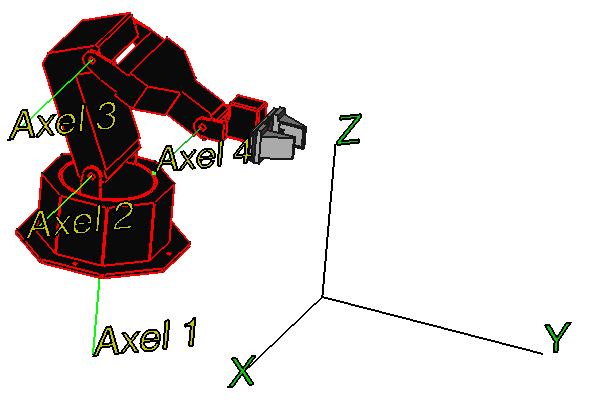
\includegraphics[scale=0.4]{grafik/robotaxis}}
\caption{\textit{Till vänster}: Armens frihetsgrader  \textit{Till höger}: Armens koordinatsystem} \label{protokoll-arm-axlar}
\end{figure}
